% !TEX root = kraft-inequality.tex
% Compile from book-sources/; see the accompanying README.
\documentclass[11pt]{article}
\usepackage[T1]{fontenc}
\usepackage[utf8]{inputenc}
\usepackage[english]{babel}
\usepackage{amsmath,amsthm}
\usepackage{newpxtext,newpxmath}
\usepackage[scaled=.94]{sourcesanspro}
\usepackage{microtype}
\usepackage[a4paper,margin=24mm,headheight=15pt,headsep=7mm]{geometry}
\usepackage{booktabs,tikz}
\usetikzlibrary{arrows.meta,patterns}
\usepackage{enumitem,fancyhdr}
\usepackage[unicode,colorlinks=true,linkcolor=teal!65!black,urlcolor=teal!65!black]{hyperref}
\input{chapters-tex/shared/book-metadata}
\definecolor{ink}{HTML}{203746}
\definecolor{accent}{HTML}{146C78}
\definecolor{muted}{HTML}{667780}
\definecolor{signalred}{HTML}{B94B44}
\definecolor{gold}{HTML}{C48A32}
\definecolor{blue}{HTML}{4778A3}
\definecolor{violet}{HTML}{78578E}
\hypersetup{pdftitle={Kraft's inequality: a detailed constructive proof},pdfauthor={\BookAuthor}}
\newtheorem{theorem}{Theorem}
\newtheorem{lemma}{Lemma}
\newcommand{\bits}{\{0,1\}}
\newcommand{\Desc}{\mathcal D}
\newcommand{\word}[1]{\texttt{#1}}
\setlength{\parindent}{0pt}
\setlength{\parskip}{5pt plus 1pt}
\setlength{\emergencystretch}{1.5em}
\setlist[enumerate]{leftmargin=*,itemsep=7pt,topsep=4pt}
\pagestyle{fancy}
\fancyhf{}
\fancyhead[L]{\small\sffamily\color{muted}Kraft's inequality}
\fancyhead[R]{\small\sffamily\color{muted}Detailed proof}
\fancyfoot[C]{\small\sffamily\thepage}
\renewcommand{\headrulewidth}{.3pt}
\raggedbottom

\begin{document}
\thispagestyle{empty}
{\sffamily\color{ink}\setlength{\parskip}{0pt}
 {\small\BookTitle\par}
 \vspace{4mm}
 {\LARGE\bfseries Kraft's inequality\par}
 \vspace{2mm}
 {\large A detailed proof of the subtree construction\par}
 \vspace{4mm}
 {\BookAuthor\hfill\small\color{muted}\BookEditionDate\par}
 {\small\color{muted}\BookAffiliation\par}
 \vspace{3mm}{\color{accent}\rule{\linewidth}{.8pt}}\par}

The converse of Kraft's inequality requires more than enough space for the
desired subtrees: their leaves must also be aligned with the branches of a
single binary tree. The construction below makes this alignment explicit.
The decisive fact is that, after the lengths have been sorted, every earlier
block size is an integer multiple of the next one.

\begin{theorem}[Kraft's inequality]
Let $K\geq1$ and let $\ell_1,\ldots,\ell_K$ be nonnegative integers.
There exist binary words $c_1,\ldots,c_K$ with $|c_k|=\ell_k$ such that,
for distinct $j,k$, $c_j$ is not a prefix of $c_k$, if and only if
\begin{equation}\label{eq:kraft}
    \sum_{k=1}^K 2^{-\ell_k}\leq1.
\end{equation}
\end{theorem}

Here, a word is a prefix of itself, so the condition also rules out assigning
the same word to two different symbols. Length zero means the empty word,
denoted by $\varepsilon$. If some $\ell_k=0$, \eqref{eq:kraft} forces $K=1$,
and the empty word gives the required code. For coding a message over that
one-symbol alphabet, its length must be supplied separately, as in the book.

\section*{Which consecutive leaves form a subtree?}

Fix $m\geq0$. Consider the complete binary tree whose vertices are all words
of length at most $m$; the children of $w$ are $w\word{0}$ and $w\word{1}$.
Its depth-$m$ leaves are the words in $\bits^m$. Number these leaves from left
to right by $0,1,\ldots,2^m-1$, using their values as binary integers.

For a word $w=w_1\cdots w_\ell$ of length $\ell\leq m$, put
\[
    q(w)=\sum_{r=1}^{\ell}w_r2^{\ell-r},
    \qquad q(\varepsilon)=0,
\]
and let $\Desc_m(w)$ be the set of indices of its depth-$m$ descendants.
Leading zeroes are part of the word even though they do not change $q(w)$.

\begin{lemma}[Aligned blocks]\label{lem:aligned}
A word $w$ of length $\ell$ has exactly the following descendant leaves:
\begin{equation}\label{eq:descendants}
 \Desc_m(w)=
 \bigl\{q(w)2^{m-\ell},\ldots,(q(w)+1)2^{m-\ell}-1\bigr\}.
\end{equation}
Consequently, a consecutive block of $b=2^{m-\ell}$ leaves, starting at index
$S$ and contained in $\{0,\ldots,2^m-1\}$, is the descendant-leaf set of a
depth-$\ell$ vertex if and only if $b$ divides $S$.
\end{lemma}

\begin{proof}
Every descendant word is obtained by appending $m-\ell$ bits to $w$.
If those appended bits represent the integer $r$, its leaf index is
$q(w)2^{m-\ell}+r$. As the appended bits vary, $r$ takes each value from
$0$ to $2^{m-\ell}-1$ exactly once, proving \eqref{eq:descendants}.

Thus a descendant block starts at a multiple of $b$. Conversely, if
$S=qb$ and the block fits, then $0\leq q<2^\ell$. Write $q$ in binary using
exactly $\ell$ bits, adding leading zeroes if necessary. Equation
\eqref{eq:descendants} shows that this word has precisely the prescribed
descendant block. For $\ell=0$, the word is $\varepsilon$ and its block
consists of all $2^m$ leaves.
\end{proof}

\section*{Proof of Kraft's inequality}

\paragraph{Necessity.}
Suppose the words are prefix-free, and set $m=\max_k\ell_k$.
The sets $\Desc_m(c_k)$ are pairwise disjoint. Indeed, if a depth-$m$ word
extended both $c_j$ and $c_k$, its two prefixes would be comparable:
the shorter would be a prefix of the longer. This contradicts prefix-freeness
when $j\ne k$.
The aligned-block lemma therefore gives
\[
 \sum_{k=1}^K 2^{m-\ell_k}
   =\sum_{k=1}^K|\Desc_m(c_k)|
   \leq 2^m.
\]
Division by $2^m$ gives \eqref{eq:kraft}.

\paragraph{Sufficiency.}
Assume \eqref{eq:kraft}. Relabel the symbols so that
\[
   \ell_1\leq\ell_2\leq\cdots\leq\ell_K,
   \qquad m=\ell_K.
\]
We will assign a vertex of the \emph{same complete depth-$m$ tree} to each
symbol. No rearrangement of the tree's branches is involved.

\begin{enumerate}[label=\textbf{\arabic*.}]
\item \textbf{Specify the blocks.}
For each $k$, define the block size and cumulative endpoints by
\begin{equation}\label{eq:blocks}
 b_k=2^{m-\ell_k},\qquad S_0=0,\qquad
 S_k=\sum_{j=1}^k b_j,
 \qquad B_k=\{S_{k-1},\ldots,S_k-1\}.
\end{equation}
These are nonempty, pairwise disjoint sets of consecutive indices.
Moreover,
\[
 S_K=2^m\sum_{k=1}^K2^{-\ell_k}\leq2^m,
\]
so every $B_k$ fits inside the leaf set of the ambient tree.

\item \textbf{Verify alignment.}
For $j<k$, the ordering gives $\ell_j\leq\ell_k$, hence
\[
 \frac{b_j}{b_k}=2^{\ell_k-\ell_j}\in\mathbb N.
\]
Thus \emph{each earlier block size is divisible by $b_k$}, and so is their
sum:
\begin{equation}\label{eq:alignment}
 \frac{S_{k-1}}{b_k}
    =\sum_{j<k}2^{\ell_k-\ell_j}\in\mathbb Z_{\geq0}.
\end{equation}
For $k=1$, the sum is empty and equals zero. This is the precise reason
that consecutive packing respects the branching structure of the tree.

\item \textbf{Turn each block into a word.}
Set $q_k=S_{k-1}/b_k$. It is an integer by \eqref{eq:alignment}, and
\[
 0\leq q_k,
 \qquad (q_k+1)b_k=S_k\leq2^m,
 \qquad\text{so}\qquad 0\leq q_k\leq2^{\ell_k}-1.
\]
There is therefore a unique word $c_k$ of exactly $\ell_k$ bits representing
$q_k$, with leading zeroes included. By Lemma~\ref{lem:aligned},
\begin{equation}\label{eq:chosen-descendants}
     \Desc_m(c_k)=B_k.
\end{equation}
This constructs actual vertices of the original complete tree, rather than
merely blocks with the correct cardinalities.

\item \textbf{Verify the prefix property.}
If $c_j$ were a prefix of $c_k$ for distinct indices, every depth-$m$
extension of $c_k$ would also extend $c_j$. Consequently,
\[
  \varnothing\ne B_k=\Desc_m(c_k)
             \subseteq\Desc_m(c_j)=B_j,
\]
contradicting the disjointness of $B_j$ and $B_k$. The words are therefore
prefix-free. Undoing the initial relabeling assigns each original symbol
a word of its prescribed length.
\end{enumerate}
This proves the converse and completes the proof of the theorem.

\paragraph{Recovering the coding tree.}
To obtain the book's representation $c=\mathrm{Leaves}(T)$, take $T$ to be
the union of the paths from the root to $c_1,\ldots,c_K$. A codeword has
no strict descendant in $T$, since otherwise it would be a prefix of
another codeword. Conversely, a vertex of $T$ that is not a codeword lies
strictly before some $c_k$ on its path and therefore has a child in $T$.
The leaves of $T$ are exactly the selected codewords. This pruned coding
tree may have vertices with only one child; it need not be complete.

\section*{A concrete example}

Take $(\ell_1,\ldots,\ell_5)=(2,2,3,4,4)$. Then $m=4$ and
$\sum_k2^{-\ell_k}=3/4$. The construction is entirely explicit:
\begin{center}
\begin{tabular}{@{}cccccc@{}}
\toprule
$k$ & $\ell_k$ & $b_k$ & $S_{k-1}$ & $q_k=S_{k-1}/b_k$ & $c_k$\\
\midrule
1 & 2 & 4 & 0 & 0 & \word{00}\\
2 & 2 & 4 & 4 & 1 & \word{01}\\
3 & 3 & 2 & 8 & 4 & \word{100}\\
4 & 4 & 1 & 10 & 10 & \word{1010}\\
5 & 4 & 1 & 11 & 11 & \word{1011}\\
\bottomrule
\end{tabular}
\end{center}

\begin{center}
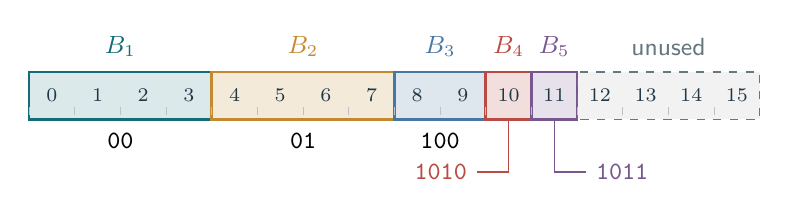
\begin{tikzpicture}[x=.58cm,y=1cm,font=\small\sffamily]
 \fill[accent!15] (0,0) rectangle (4,.6);
 \fill[gold!18] (4,0) rectangle (8,.6);
 \fill[blue!18] (8,0) rectangle (10,.6);
 \fill[signalred!18] (10,0) rectangle (11,.6);
 \fill[violet!18] (11,0) rectangle (12,.6);
 \fill[black!5] (12,0) rectangle (16,.6);
 \foreach \a/\b/\c in {0/4/accent,4/8/gold,8/10/blue,10/11/signalred,11/12/violet}
   \draw[\c,line width=1pt] (\a,0) rectangle (\b,.6);
 \draw[muted,dashed] (12,0) rectangle (16,.6);
 \foreach \j in {0,...,15} {
   \draw[muted!45] (\j,.05)--(\j,.15);
   \node[font=\scriptsize,text=ink] at (\j+.5,.30) {\j};
 }
 \node[text=accent] at (2,.92) {$B_1$};
 \node[text=gold] at (6,.92) {$B_2$};
 \node[text=blue] at (9,.92) {$B_3$};
 \node[text=signalred] at (10.5,.92) {$B_4$};
 \node[text=violet] at (11.5,.92) {$B_5$};
 \node[text=muted] at (14,.92) {unused};
 \node at (2,-.28) {\word{00}};
 \node at (6,-.28) {\word{01}};
 \node at (9,-.28) {\word{100}};
 \draw[signalred] (10.5,0)--(10.5,-.67)--(9.8,-.67);
 \node[anchor=east,text=signalred] at (9.8,-.67) {\word{1010}};
 \draw[violet] (11.5,0)--(11.5,-.67)--(12.2,-.67);
 \node[anchor=west,text=violet] at (12.2,-.67) {\word{1011}};
\end{tikzpicture}
\end{center}

Each colored block contains the depth-$4$ extensions of the word written
below it. In particular, $B_3=\{8,9\}$ corresponds to the vertex
$\word{100}$, since its extensions are $\word{1000}$ and $\word{1001}$.
The four unused leaves cause no difficulty: Kraft's inequality does not
require that every leaf of the ambient tree be assigned to a codeword.

\paragraph{Why the sorting matters.}
For lengths $(3,1)$, the Kraft sum is $5/8$, so a code exists. However, at
depth $m=3$, packing blocks in that order gives $\{0\}$ followed by
$\{1,2,3,4\}$. The latter block is not the descendant set of a depth-$1$
vertex: the only such blocks are $\{0,1,2,3\}$ and $\{4,5,6,7\}$.
Sorting the lengths as $(1,3)$ gives blocks $\{0,1,2,3\}$ and $\{4\}$,
corresponding to $\word{0}$ and $\word{100}$. They can then be reassigned
to the original symbols in the required order.

\section*{An alternative inductive proof of the converse}

The same argument can be phrased without consecutive blocks. After sorting
the lengths, suppose that prefix-free words $c_1,\ldots,c_{k-1}$ of the
prescribed lengths have been chosen. At depth $\ell_k$, the extensions of
$c_j$ occupy exactly $2^{\ell_k-\ell_j}$ vertices. These forbidden sets
are disjoint, because the previously chosen words are prefix-free. Hence
the number of available vertices is
\[
 A_k=2^{\ell_k}-\sum_{j<k}2^{\ell_k-\ell_j}.
\]
The partial Kraft inequality gives
\[
 \sum_{j<k}2^{-\ell_j}+2^{-\ell_k}\leq1,
 \qquad\text{and therefore}\qquad A_k\geq1.
\]
Choose an available word at depth $\ell_k$. It cannot extend any previous
codeword, by availability. It cannot be a prefix of one either: all previous
lengths are at most $\ell_k$, and equality of words is also excluded by
availability. Thus the enlarged family is prefix-free, and induction
constructs all $K$ codewords.

This version separates the two ingredients particularly clearly: sorted
lengths prevent a newly chosen word from sitting above an earlier one,
and Kraft's inequality guarantees a free vertex at every step.

\end{document}
